\documentclass[tikz,border=10pt]{standalone}
\usetikzlibrary{decorations.pathreplacing, calc}

\begin{document}

% Reduced x-scale slightly to fit the wider 2N=16 period
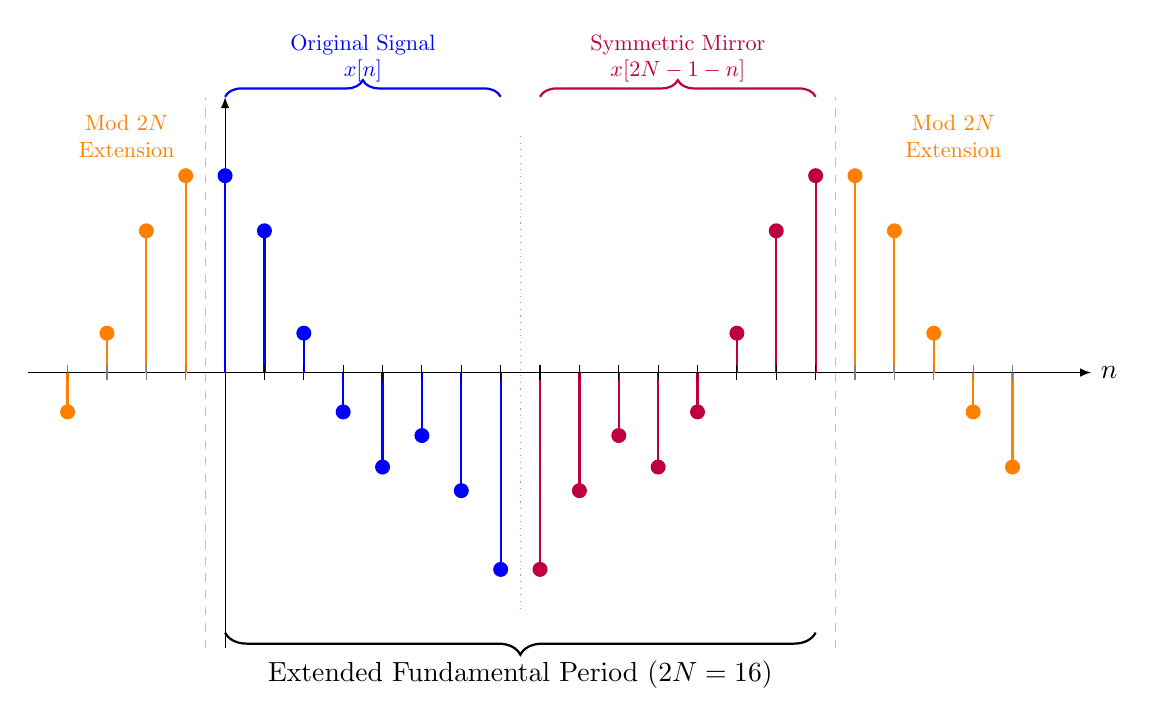
\begin{tikzpicture}[>=latex, x=0.5cm, y=1.0cm]

% --- Configuration ---
\def\N{8} 
\def\TwoN{16}

% Define ORIGINAL signal values for indices 0 to 7
\def\vzero{2.5}
\def\vone{1.8}
\def\vtwo{0.5}
\def\vthree{-0.5}
\def\vfour{-1.2}
\def\vfive{-0.8}
\def\vsix{-1.5}
\def\vseven{-2.5}

% --- Draw Axis ---
% Range: -5 to 21 (covers period 0 and small parts of neighbors)
\draw[->] (-5,0) -- (22,0) node[right] {$n$};
\draw[->] (0,-3.5) -- (0,3.5); % Vertical axis

% --- Main Loop ---
% We iterate through absolute indices n from -4 to 20
\foreach \n in {-4, ..., 20} {
    
    % 1. Calculate the Modulo 2N index (0 to 15)
    % Logic: ((n % 16) + 16) % 16 handles negative n correctly
    \pgfmathtruncatemacro{\modidx}{mod(mod(\n, \TwoN) + \TwoN, \TwoN)}
    
    % 2. Determine value based on Mirroring Logic
    % If index < 8, use original. If index >= 8, use mirrored (15-index).
    \pgfmathtruncatemacro{\lookupidx}{(\modidx < \N) ? \modidx : (2*\N - 1 - \modidx)}
    
    % Fetch value
    \ifcase\lookupidx
        \let\val\vzero
    \or
        \let\val\vone
    \or
        \let\val\vtwo
    \or
        \let\val\vthree
    \or
        \let\val\vfour
    \or
        \let\val\vfive
    \or
        \let\val\vsix
    \or
        \let\val\vseven
    \fi
    
    % 3. Determine Region and Color
    \ifnum\n<0
        % Left Extension (Orange)
        \draw[thick, orange] (\n,0) -- (\n,\val);
        \filldraw[orange] (\n,\val) circle (2.5pt);
        \draw[gray] (\n, 0.1) -- (\n, -0.1);
    \else
        \ifnum\n>15
            % Right Extension (Orange)
            \draw[thick, orange] (\n,0) -- (\n,\val);
            \filldraw[orange] (\n,\val) circle (2.5pt);
            \draw[gray] (\n, 0.1) -- (\n, -0.1);
        \else
            % FUNDAMENTAL PERIOD (0 to 15)
            \ifnum\n<8
                % Original Signal (Blue)
                \draw[thick, blue] (\n,0) -- (\n,\val);
                \filldraw[blue] (\n,\val) circle (2.5pt);
                \draw (\n, 0.1) -- (\n, -0.1);
            \else
                % Mirrored Part (Purple)
                \draw[thick, purple] (\n,0) -- (\n,\val);
                \filldraw[purple] (\n,\val) circle (2.5pt);
                \draw (\n, 0.1) -- (\n, -0.1);
            \fi
        \fi
    \fi
}

% --- Visual Separators ---
\draw[dashed, lightgray] (-0.5, -3.5) -- (-0.5, 3.5);   % Start of Period
\draw[dashed, lightgray] (15.5, -3.5) -- (15.5, 3.5);   % End of Period
\draw[dotted, purple!50] (7.5, -3.0) -- (7.5, 3.0);     % Mirror axis

% --- Annotations ---

% 1. Original
\draw[decoration={brace,amplitude=6pt,raise=2ex},decorate,thick, blue] 
  (0,3.2) -- (7,3.2) 
  node[midway,above=2.5ex, align=center, blue, scale=0.8] {Original Signal\\$x[n]$};

% 2. Mirror
\draw[decoration={brace,amplitude=6pt,raise=2ex},decorate,thick, purple] 
  (8,3.2) -- (15,3.2) 
  node[midway,above=2.5ex, align=center, purple, scale=0.8] {Symmetric Mirror\\$x[2N-1-n]$};

% 3. Total Period
\draw[decoration={brace,amplitude=8pt,raise=2ex, mirror},decorate,thick, black] 
  (0,-3) -- (15,-3) 
  node[midway,below=3.5ex, align=center, black] {Extended Fundamental Period ($2N=16$)};

% 4. Extension Labels
\node[orange, scale=0.8, align=center] at (-2.5, 3) {Mod $2N$\\Extension};
\node[orange, scale=0.8, align=center] at (18.5, 3) {Mod $2N$\\Extension};

\end{tikzpicture}
\end{document}